% Chapter 6: Seminar - VAR Models and Granger Causality
% Quizzes, Practice Problems, and Discussion
% Bachelor program, Bucharest University of Economic Studies

\documentclass[9pt, aspectratio=169, t]{beamer}

% Ensure content fits on slides
\setbeamersize{text margin left=8mm, text margin right=8mm}

%=============================================================================
% THEME AND STYLE CONFIGURATION
%=============================================================================
\usetheme{default}
% Using default theme for clean header/footer control

% Color Palette (matching Redispatch PDF)
\definecolor{MainBlue}{RGB}{26, 58, 110}
\definecolor{AccentBlue}{RGB}{26, 58, 110}
\definecolor{IDAred}{RGB}{205, 0, 0}
\definecolor{DarkGray}{RGB}{51, 51, 51}
\definecolor{MediumGray}{RGB}{128, 128, 128}
\definecolor{LightGray}{RGB}{248, 248, 248}
\definecolor{VeryLightGray}{RGB}{235, 235, 235}
\definecolor{KeynoteGray}{RGB}{218, 218, 218}
\definecolor{SectionGray}{RGB}{120, 120, 120}
\definecolor{FooterGray}{RGB}{100, 100, 100}
\definecolor{Crimson}{RGB}{220, 53, 69}
\definecolor{Forest}{RGB}{46, 125, 50}
\definecolor{Amber}{RGB}{181, 133, 63}
\definecolor{Orange}{RGB}{230, 126, 34}
\definecolor{Purple}{RGB}{142, 68, 173}

% Gradient background (exact Keynote 315° gradient: white to RGB 218,218,218)
\setbeamertemplate{background}{%
    \begin{tikzpicture}[remember picture, overlay]
        \shade[shading=axis, shading angle=315,
        top color=white, bottom color=KeynoteGray]
        (current page.south west) rectangle (current page.north east);
    \end{tikzpicture}%
}
% Fallback solid color for compatibility
\setbeamercolor{background canvas}{bg=}

\setbeamercolor{palette primary}{bg=MainBlue, fg=white}
\setbeamercolor{palette secondary}{bg=MainBlue!85, fg=white}
\setbeamercolor{palette tertiary}{bg=MainBlue!70, fg=white}
\setbeamercolor{structure}{fg=MainBlue}
\setbeamercolor{title}{fg=IDAred}
\setbeamercolor{frametitle}{fg=IDAred, bg=}
\setbeamercolor{block title}{bg=MainBlue, fg=white}
\setbeamercolor{block body}{bg=VeryLightGray, fg=DarkGray}
\setbeamercolor{block title alerted}{bg=Crimson, fg=white}
\setbeamercolor{block body alerted}{bg=Crimson!8, fg=DarkGray}
\setbeamercolor{block title example}{bg=Forest, fg=white}
\setbeamercolor{block body example}{bg=Forest!8, fg=DarkGray}
\setbeamercolor{item}{fg=MainBlue}

% Footer colors (override Madrid theme blue)
\setbeamercolor{author in head/foot}{fg=FooterGray, bg=}
\setbeamercolor{title in head/foot}{fg=FooterGray, bg=}
\setbeamercolor{date in head/foot}{fg=FooterGray, bg=}
\setbeamercolor{section in head/foot}{fg=FooterGray, bg=}
\setbeamercolor{subsection in head/foot}{fg=FooterGray, bg=}

% Bullet styles (apply everywhere including blocks)
\setbeamertemplate{itemize item}{\color{MainBlue}$\boxdot$}
\setbeamertemplate{itemize subitem}{\color{MainBlue}$\blacktriangleright$}
\setbeamertemplate{itemize subsubitem}{\color{MainBlue}\tiny$\bullet$}
\setbeamertemplate{itemize/enumerate body begin}{\normalsize}
\setbeamertemplate{itemize/enumerate subbody begin}{\normalsize}

% Item spacing - compact style
\setlength{\leftmargini}{10pt}       % Level 1: minimal indent
\setlength{\leftmarginii}{10pt}      % Level 2: minimal additional indent
% Compact list spacing (zero extra space before/after lists in blocks)
\makeatletter
\def\@listi{\leftmargin\leftmargini \topsep 0pt \parsep 0pt \itemsep 0pt}
\def\@listii{\leftmargin\leftmarginii \topsep 0pt \parsep 0pt \itemsep 0pt}
\makeatother

\setbeamertemplate{navigation symbols}{}

%=============================================================================
% CUSTOM HEADLINE
%=============================================================================
\setbeamertemplate{headline}{%
    \vskip10pt%
    \hbox to \paperwidth{%
        \hskip0.5cm%
        {\small\color{FooterGray}\renewcommand{\hyperlink}[2]{##2}\insertsectionhead}%
        \hfill%
        \textcolor{FooterGray}{\small\insertframenumber}%
        \hskip0.5cm%
    }%
    \vskip4pt%
    {\color{FooterGray}\hrule height 0.4pt}%
}

%=============================================================================
% CUSTOM FOOTER
%=============================================================================
\usepackage{fontawesome5}

\setbeamertemplate{footline}{%
    {\color{FooterGray}\hrule height 0.4pt}%
    \vskip4pt%
    \hbox to \paperwidth{%
        \hskip0.5cm%
        \textcolor{FooterGray}{\small Time Series Analysis and Forecasting}%
        \hfill%
        \raisebox{-0.1em}{%
            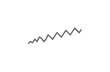
\begin{tikzpicture}[x=0.08em, y=0.08em, line width=0.4pt]
                \draw[FooterGray] (0,3) -- (1,4) -- (2,3.5) -- (3,5) -- (4,4) -- (5,6) -- (6,5.5) -- (7,4) -- (8,5) -- (9,7) -- (10,6) -- (11,5) -- (12,6.5) -- (13,8) -- (14,7) -- (15,6) -- (16,7.5) -- (17,9) -- (18,8) -- (19,7) -- (20,8.5) -- (21,10) -- (22,9) -- (23,8) -- (24,9.5);
            \end{tikzpicture}%
        }%
        \hskip0.5cm%
    }%
    \vskip6pt%
}

%=============================================================================
% PACKAGES
%=============================================================================
\usepackage[utf8]{inputenc}
\usepackage[T1]{fontenc}
\usepackage[english]{babel}
\usepackage{amsmath, amssymb, amsthm}
\usepackage{mathtools}
\usepackage{bm}
\usepackage{tikz}
\usetikzlibrary{arrows.meta, positioning, shapes, calc, decorations.pathreplacing, shadings}
\usepackage{booktabs}
\usepackage{multirow}
\usepackage{array}
\usepackage{graphicx}
\usepackage{hyperref}
\usepackage{colortbl}
\hypersetup{colorlinks=true, linkcolor=MainBlue, urlcolor=MainBlue}
\graphicspath{{../../logos/}{../../charts/}}
\hfuzz=2pt  % Suppress tiny overfull warnings (<2pt)
\vfuzz=2pt  % Suppress tiny vertical overfull warnings (<2pt)

%=============================================================================
% CENTRED MINIPAGE
%=============================================================================
\newenvironment{cminipage}[1]{%
    \par\noindent\hfill\begin{minipage}{#1}\ignorespaces
}{%
    \end{minipage}\hfill\null\par
}

%=============================================================================
% QUANTLET COMMAND
%=============================================================================
\newcommand{\quantlet}[2]{%
    \hfill\href{#2}{%
        \raisebox{-0.15em}{\includegraphics[height=0.7em]{ql_logo.png}}%
        \textcolor{MainBlue}{\tiny\ #1}%
    }%
}

%=============================================================================
% CUSTOM COMMANDS
%=============================================================================
\newcommand{\E}{\mathbb{E}}
\newcommand{\Var}{\text{Var}}
\newcommand{\Cov}{\text{Cov}}
\newcommand{\bY}{\mathbf{Y}}
\newcommand{\bA}{\mathbf{A}}
\newcommand{\bepsilon}{\boldsymbol{\varepsilon}}
\newcommand{\bvarepsilon}{\boldsymbol{\varepsilon}}
\newcommand{\bc}{\mathbf{c}}

%=============================================================================
% TITLE INFORMATION
%=============================================================================
\title[Chapter 6: Seminar]{Chapter 6: Seminar --- VAR \& Granger Causality}
\subtitle{Bachelor program Faculty of Cybernetics, Statistics and Economic Informatics, Bucharest University of Economic Studies, Romania}
\author[Prof. dr. Daniel Traian Pele]{Prof. dr. Daniel Traian Pele\\[0.2cm]\footnotesize\texttt{danpele@ase.ro}}
\institute{Bucharest University of Economic Studies}
\date{Academic Year 2025--2026}

\begin{document}

%=============================================================================
% TITLE SLIDE
%=============================================================================
\begin{frame}[plain]
    \begin{tikzpicture}[remember picture, overlay]
        \fill[IDAred] (current page.north west) rectangle ([yshift=-0.15cm]current page.north east);
        \node[anchor=north west] at ([xshift=0.5cm, yshift=-0.3cm]current page.north west) {
            \href{https://www.ase.ro}{\includegraphics[height=1.1cm]{ase_logo.png}}
        };
        \node[anchor=north] at ([yshift=-0.3cm]current page.north) {
            \href{https://ai4efin.ase.ro}{\includegraphics[height=1.1cm]{ai4efin_logo.png}}
        };
        \node[anchor=north east] at ([xshift=-0.5cm, yshift=-0.3cm]current page.north east) {
            \href{https://www.digital-finance-msca.com}{\includegraphics[height=1.1cm]{msca_logo.png}}
        };
    \end{tikzpicture}
    \vfill
    \begin{center}
        {\Large\textcolor{MediumGray}{Time Series Analysis and Forecasting}}\\[0.3cm]
        {\Huge\textbf{\textcolor{MainBlue}{Chapter 6: VAR \& Granger Causality}}}\\[0.5cm]
        {\Large\textcolor{IDAred}{Seminar}}
    \end{center}
    \vfill

    \begin{tikzpicture}[remember picture, overlay]
        \fill[IDAred] (current page.south west) rectangle ([yshift=0.15cm]current page.south east);
        \node[anchor=south west] at ([xshift=0.5cm, yshift=0.8cm]current page.south west) {
            \href{https://theida.net}{\includegraphics[height=0.9cm]{ida_logo.png}}
        };
        \node[anchor=south] at ([xshift=-3cm, yshift=0.8cm]current page.south) {
            \href{https://blockchain-research-center.com}{\includegraphics[height=0.9cm]{brc_logo.png}}
        };
        \node[anchor=south] at ([yshift=0.8cm]current page.south) {
            \href{https://quantinar.com}{\includegraphics[height=0.9cm]{qr_logo.png}}
        };
        \node[anchor=south] at ([xshift=3cm, yshift=0.8cm]current page.south) {
            \href{https://quantlet.com}{\includegraphics[height=0.9cm]{ql_logo.png}}
        };
        \node[anchor=south east] at ([xshift=-0.5cm, yshift=0.8cm]current page.south east) {
            \href{https://ipe.ro/new}{\includegraphics[height=0.9cm]{acad_logo.png}}
        };
    \end{tikzpicture}
\end{frame}

%=============================================================================
% OUTLINE
%=============================================================================
\begin{frame}{Seminar Outline}
    \begin{cminipage}{0.95\textwidth}
    \textbf{\large Seminar structure:}

    \vspace{0.4cm}

    \begin{enumerate}
        \item[\textcolor{MainBlue}{\textbf{1.}}] \textbf{Review Quiz} -- Knowledge check
        \vspace{0.15cm}
        \item[\textcolor{MainBlue}{\textbf{2.}}] \textbf{True/False Questions} -- Conceptual checks
        \vspace{0.15cm}
        \item[\textcolor{MainBlue}{\textbf{3.}}] \textbf{Practice Problems} -- Applied practice
        \vspace{0.15cm}
        \item[\textcolor{MainBlue}{\textbf{4.}}] \textbf{Worked Examples} -- Detailed solutions
        \vspace{0.15cm}
        \item[\textcolor{MainBlue}{\textbf{5.}}] \textbf{Real Data Analysis} -- Empirical applications
        \vspace{0.15cm}
        \item[\textcolor{MainBlue}{\textbf{6.}}] \textbf{Discussion Topics} -- Critical thinking
        \vspace{0.15cm}
        \item[\textcolor{MainBlue}{\textbf{7.}}] \textbf{AI-Assisted Exercises} -- Applied artificial intelligence
    \end{enumerate}
    \end{cminipage}
\end{frame}

%=============================================================================
% SECTION 1: REVIEW QUIZ
%=============================================================================
\section{Review Quiz}

\begin{frame}{Quiz 1: VAR Definition}
    \begin{alertblock}{Question}
        In a VAR(2) model with 3 variables, how many coefficient matrices $\bA_i$ are there?
    \end{alertblock}

    \vspace{0.3cm}

    \begin{enumerate}[A)]
        \item 2
        \item 3
        \item 6
        \item 9
    \end{enumerate}

    \vspace{0.5cm}
    \begin{flushright}\textit{Answer on next slide...}\end{flushright}
\end{frame}

\begin{frame}{Quiz 1: Answer}
    \begin{exampleblock}{Answer: A -- 2 coefficient matrices}
        \textbf{VAR($p$) model}: $\bY_t = \bc + \bA_1\bY_{t-1} + \bA_2\bY_{t-2} + \cdots + \bA_p\bY_{t-p} + \bvarepsilon_t$

        \vspace{0.3cm}
        \textbf{VAR(2) with $K=3$}:
        \[
        \begin{pmatrix} Y_{1t} \\ Y_{2t} \\ Y_{3t} \end{pmatrix} = \bc + \underbrace{\bA_1}_{3\times 3}\begin{pmatrix} Y_{1,t-1} \\ Y_{2,t-1} \\ Y_{3,t-1} \end{pmatrix} + \underbrace{\bA_2}_{3\times 3}\begin{pmatrix} Y_{1,t-2} \\ Y_{2,t-2} \\ Y_{3,t-2} \end{pmatrix} + \bvarepsilon_t
        \]

        \textbf{Key}: $p$ = number of lags = number of matrices
    \end{exampleblock}
    \quantlet{TSA\_ch6\_var\_basics}{https://github.com/QuantLet/TSA/tree/main/TSA_ch6/TSA_ch6_var_basics}
\end{frame}

\begin{frame}{Quiz 2: Number of Parameters}
    \begin{alertblock}{Question}
        A VAR(2) with $K=3$ variables (including constants) has how many parameters to estimate per equation?
    \end{alertblock}

    \vspace{0.3cm}

    \begin{enumerate}[A)]
        \item 3
        \item 6
        \item 7
        \item 9
    \end{enumerate}

    \vspace{0.5cm}
    \begin{flushright}\textit{Answer on next slide...}\end{flushright}
\end{frame}

\begin{frame}{Quiz 2: Answer}
    \begin{exampleblock}{Answer: C -- 7 parameters per equation}
        \begin{center}
            \includegraphics[width=0.95\textwidth, height=0.55\textheight, keepaspectratio]{sem5_var_parameters.pdf}
        \end{center}
        \vspace{-0.2cm}
        {\footnotesize
        \textbf{Formula}: Per equation = $1 + K \times p = 1 + 3 \times 2 = 7$. \textbf{Total}: $K(1 + Kp) = 3(1 + 6) = 21$ parameters
        }
    \end{exampleblock}
    \quantlet{TSA\_ch6\_var\_estimation}{https://github.com/QuantLet/TSA/tree/main/TSA_ch6/TSA_ch6_var_estimation}
\end{frame}

\begin{frame}{Quiz 3: Granger Causality}
    \begin{alertblock}{Question}
        ``$X$ Granger-causes $Y$'' means:
    \end{alertblock}

    \vspace{0.3cm}

    \begin{enumerate}[A)]
        \item $X$ is the economic cause of $Y$
        \item Past $X$ helps predict future $Y$
        \item $X$ and $Y$ are contemporaneously correlated
        \item $X$ always increases when $Y$ increases
    \end{enumerate}

    \vspace{0.5cm}
    \begin{flushright}\textit{Answer on next slide...}\end{flushright}
\end{frame}

\begin{frame}{Quiz 3: Answer}
    \begin{exampleblock}{Answer: B -- Past $X$ helps predict future $Y$}
        \begin{center}
            \includegraphics[width=0.9\textwidth, height=0.55\textheight, keepaspectratio]{sem5_granger_diagram.pdf}
        \end{center}
        \vspace{-0.2cm}
        {\footnotesize
        \textbf{Key}: Predictive relationship, NOT true causation!
        }
    \end{exampleblock}
    \quantlet{TSA\_ch6\_granger}{https://github.com/QuantLet/TSA/tree/main/TSA_ch6/TSA_ch6_granger}
\end{frame}

\begin{frame}{Quiz 4: Granger Causality Test}
    \begin{alertblock}{Question}
        To test if $Y_2$ Granger-causes $Y_1$ in a VAR(p), we test:
    \end{alertblock}

    \vspace{0.3cm}

    \begin{enumerate}[A)]
        \item All coefficients in the $Y_1$ equation equal zero
        \item Coefficients on lagged $Y_2$ in the $Y_1$ equation equal zero
        \item Coefficients on lagged $Y_1$ in the $Y_2$ equation equal zero
        \item The error covariance equals zero
    \end{enumerate}

    \vspace{0.5cm}
    \begin{flushright}\textit{Answer on next slide...}\end{flushright}
\end{frame}

\begin{frame}{Quiz 4: Answer}
    \begin{exampleblock}{Answer: B -- Coefficients on lagged $Y_2$ in $Y_1$ equation = 0}
        \textbf{Null hypothesis}: $H_0: a_{12}^{(1)} = a_{12}^{(2)} = \cdots = a_{12}^{(p)} = 0$

        \vspace{0.2cm}
        \textbf{Test statistic}: Wald or F-test with $p$ restrictions

        \vspace{0.2cm}
        \textbf{Interpretation}:
        \begin{itemize}
            \item Reject $H_0$: $Y_2$ Granger-causes $Y_1$
            \item Don't reject: No evidence of predictive relationship
        \end{itemize}

        \vspace{0.2cm}
        \textbf{Note}: Test $Y_1 \to Y_2$ separately (different coefficients in $Y_2$ equation)
    \end{exampleblock}
\end{frame}

\begin{frame}{Quiz 5: VAR Stability}
    \begin{alertblock}{Question}
        A VAR(1) model is stable (stationary) if:
    \end{alertblock}

    \vspace{0.3cm}

    \begin{enumerate}[A)]
        \item All diagonal elements of $\bA_1$ are less than 1
        \item The determinant of $\bA_1$ is less than 1
        \item All eigenvalues of $\bA_1$ are less than 1 in absolute value
        \item The trace of $\bA_1$ equals zero
    \end{enumerate}

    \vspace{0.5cm}
    \begin{flushright}\textit{Answer on next slide...}\end{flushright}
\end{frame}

\begin{frame}{Quiz 5: Answer}
    \begin{exampleblock}{Answer: C -- All eigenvalues of $\bA_1$ inside unit circle}
        \begin{center}
            \includegraphics[width=0.95\textwidth, height=0.6\textheight, keepaspectratio]{sem5_var_stability.pdf}
        \end{center}
        \vspace{-0.2cm}
        {\footnotesize
        \textbf{Stable}: All $|\lambda_i| < 1$ (inside unit circle) $\Rightarrow$ shocks die out over time
        }
    \end{exampleblock}
    \quantlet{TSA\_ch6\_var\_basics}{https://github.com/QuantLet/TSA/tree/main/TSA_ch6/TSA_ch6_var_basics}
\end{frame}

\begin{frame}{Quiz 6: Impulse Response Functions}
    \begin{alertblock}{Question}
        An impulse response function shows:
    \end{alertblock}

    \vspace{0.3cm}

    \begin{enumerate}[A)]
        \item The correlation between two variables
        \item The effect of a shock to one variable on all variables over time
        \item The forecast accuracy of the model
        \item The p-values of coefficient tests
    \end{enumerate}

    \vspace{0.5cm}
    \begin{flushright}\textit{Answer on next slide...}\end{flushright}
\end{frame}

\begin{frame}{Quiz 6: Answer}
    \begin{exampleblock}{Answer: B -- Effect of shock on all variables over time}
        \begin{center}
            \includegraphics[width=0.95\textwidth, height=0.6\textheight, keepaspectratio]{sem5_irf_example.pdf}
        \end{center}
        \vspace{-0.2cm}
        {\footnotesize
        \textbf{IRF}$_{ij}(h)$: Response of variable $i$ at horizon $h$ to shock in variable $j$
        }
    \end{exampleblock}
    \quantlet{TSA\_ch6\_irf}{https://github.com/QuantLet/TSA/tree/main/TSA_ch6/TSA_ch6_irf}
\end{frame}

\begin{frame}{Quiz 7: Lag Order Selection}
    \begin{alertblock}{Question}
        Which criterion typically selects the most parsimonious VAR model?
    \end{alertblock}

    \vspace{0.3cm}

    \begin{enumerate}[A)]
        \item AIC (Akaike Information Criterion)
        \item BIC (Bayesian Information Criterion)
        \item FPE (Final Prediction Error)
        \item Adjusted $R^2$
    \end{enumerate}

    \vspace{0.5cm}
    \begin{flushright}\textit{Answer on next slide...}\end{flushright}
\end{frame}

\begin{frame}{Quiz 7: Answer}
    \begin{exampleblock}{Answer: B -- BIC (Bayesian Information Criterion)}
        \textbf{Penalty comparison} (for $k$ parameters, $n$ observations):
        \begin{itemize}
            \item AIC: $-2\ln L + 2k$
            \item BIC: $-2\ln L + k\ln n$
        \end{itemize}

        Since $\ln n > 2$ for $n > 8$, BIC penalizes complexity more heavily

        \vspace{0.2cm}
        \textbf{Practical guidance}:
        \begin{itemize}
            \item Forecasting: AIC may perform better
            \item Inference/parsimony: BIC preferred
            \item Large samples: BIC consistent, AIC tends to overfit
        \end{itemize}
    \end{exampleblock}
    \quantlet{TSA\_ch6\_var\_selection}{https://github.com/QuantLet/TSA/tree/main/TSA_ch6/TSA_ch6_var_selection}
\end{frame}

\begin{frame}{Quiz 8: Interpreting Granger Causality}
    \begin{alertblock}{Question}
        ``$X$ Granger-causes $Y$'' means:
    \end{alertblock}

    \vspace{0.3cm}

    \begin{enumerate}[A)]
        \item $X$ is the true cause of $Y$
        \item Past values of $X$ help predict $Y$ beyond $Y$'s own past
        \item $X$ and $Y$ are correlated
        \item $Y$ depends only on $X$
    \end{enumerate}

    \vspace{0.5cm}
    \begin{flushright}\textit{Answer on next slide...}\end{flushright}
\end{frame}

\begin{frame}{Quiz 8: Answer}
    \begin{exampleblock}{Answer: B}
        Granger causality refers to \textbf{predictive} content, not true causation. $X$ Granger-causes $Y$ if lagged $X$ terms are jointly significant in the $Y$ equation, after controlling for lagged $Y$.
    \end{exampleblock}
\end{frame}

\begin{frame}{Quiz 9: Forecast Error Variance Decomposition}
    \begin{alertblock}{Question}
        FEVD (Forecast Error Variance Decomposition) tells us:
    \end{alertblock}

    \vspace{0.3cm}

    \begin{enumerate}[A)]
        \item The correlation between variables
        \item What proportion of forecast error variance comes from each shock
        \item The optimal forecast horizon
        \item Which variables to include in the model
    \end{enumerate}

    \vspace{0.5cm}
    \begin{flushright}\textit{Answer on next slide...}\end{flushright}
\end{frame}

\begin{frame}{Quiz 9: Answer}
    \begin{exampleblock}{Answer: B -- Proportion of forecast error variance from each shock}
        \begin{center}
            \includegraphics[width=0.95\textwidth, height=0.6\textheight, keepaspectratio]{sem5_fevd_example.pdf}
        \end{center}
        \vspace{-0.2cm}
        {\footnotesize
        \textbf{FEVD}: Shows how much forecast uncertainty comes from each shock at different horizons
        }
    \end{exampleblock}
    \quantlet{TSA\_ch6\_fevd}{https://github.com/QuantLet/TSA/tree/main/TSA_ch6/TSA_ch6_fevd}
\end{frame}

\begin{frame}{Quiz 10: Structural vs Reduced Form VAR}
    \begin{alertblock}{Question}
        The difference between structural VAR (SVAR) and reduced-form VAR is:
    \end{alertblock}

    \vspace{0.3cm}

    \begin{enumerate}[A)]
        \item SVAR has more variables
        \item SVAR allows contemporaneous effects between variables
        \item SVAR uses different estimation methods
        \item There is no difference
    \end{enumerate}

    \vspace{0.5cm}
    \begin{flushright}\textit{Answer on next slide...}\end{flushright}
\end{frame}

\begin{frame}{Quiz 10: Answer}
    \begin{exampleblock}{Answer: B}
        Reduced-form VAR: shocks are correlated, no contemporaneous effects in equations. SVAR: imposes identifying restrictions to recover structural shocks with economic interpretation (e.g., monetary policy shock).
    \end{exampleblock}
\end{frame}

\begin{frame}{Quiz 11: Cholesky Decomposition}
    \begin{alertblock}{Question}
        Cholesky ordering in IRF analysis assumes:
    \end{alertblock}

    \vspace{0.3cm}

    \begin{enumerate}[A)]
        \item All variables are equally important
        \item Variables ordered first affect later variables contemporaneously, not vice versa
        \item Shocks are uncorrelated
        \item No restrictions are needed
    \end{enumerate}

    \vspace{0.5cm}
    \begin{flushright}\textit{Answer on next slide...}\end{flushright}
\end{frame}

\begin{frame}{Quiz 11: Answer}
    \begin{exampleblock}{Answer: B -- Variables ordered first affect later ones contemporaneously}
        \begin{center}
            \includegraphics[width=0.95\textwidth, height=0.6\textheight, keepaspectratio]{sem5_cholesky_ordering.pdf}
        \end{center}
        \vspace{-0.2cm}
        {\footnotesize
        \textbf{Cholesky}: Recursive structure. Ordering matters -- justify by economic theory (most exogenous first)!
        }
    \end{exampleblock}
\end{frame}

\begin{frame}{Quiz 12: VAR Residual Diagnostics}
    \begin{alertblock}{Question}
        In a well-specified VAR, residuals should be:
    \end{alertblock}

    \vspace{0.3cm}

    \begin{enumerate}[A)]
        \item Autocorrelated but homoskedastic
        \item White noise (no autocorrelation)
        \item Normally distributed only
        \item Correlated across equations
    \end{enumerate}

    \vspace{0.5cm}
    \begin{flushright}\textit{Answer on next slide...}\end{flushright}
\end{frame}

\begin{frame}{Quiz 12: Answer}
    \begin{exampleblock}{Answer: B -- White noise (no autocorrelation)}
        \begin{center}
            \includegraphics[width=0.95\textwidth, height=0.6\textheight, keepaspectratio]{sem5_var_diagnostics.pdf}
        \end{center}
        \vspace{-0.2cm}
        {\footnotesize
        \textbf{Diagnostics}: Residuals should be white noise. Use Portmanteau/LM test. Cross-equation correlation allowed ($\Sigma_u$).
        }
    \end{exampleblock}
    \quantlet{TSA\_ch6\_var\_diagnostics}{https://github.com/QuantLet/TSA/tree/main/TSA_ch6/TSA_ch6_var_diagnostics}
\end{frame}

\begin{frame}{Quiz 13: Cointegration and VAR}
    \begin{alertblock}{Question}
        If variables are I(1) and cointegrated, you should use:
    \end{alertblock}

    \vspace{0.3cm}

    \begin{enumerate}[A)]
        \item VAR in levels
        \item VAR in first differences
        \item Vector Error Correction Model (VECM)
        \item Univariate ARIMA models
    \end{enumerate}

    \vspace{0.5cm}
    \begin{flushright}\textit{Answer on next slide...}\end{flushright}
\end{frame}

\begin{frame}{Quiz 13: Answer}
    \begin{exampleblock}{Answer: C}
        With cointegration, VAR in differences loses long-run information, while VAR in levels may be inefficient. VECM incorporates both short-run dynamics and long-run equilibrium relationships through the error correction term.
    \end{exampleblock}
\end{frame}

\begin{frame}{Quiz 14: Instantaneous Causality}
    \begin{alertblock}{Question}
        Instantaneous causality differs from Granger causality because it tests:
    \end{alertblock}

    \vspace{0.3cm}

    \begin{enumerate}[A)]
        \item Lagged relationships only
        \item Contemporaneous correlation of residuals
        \item Long-run relationships
        \item Model stability
    \end{enumerate}

    \vspace{0.5cm}
    \begin{flushright}\textit{Answer on next slide...}\end{flushright}
\end{frame}

\begin{frame}{Quiz 14: Answer}
    \begin{exampleblock}{Answer: B}
        Instantaneous causality tests whether shocks to $X$ and $Y$ are correlated within the same period (correlation of VAR residuals). Granger causality tests whether \textit{lagged} values help predict.
    \end{exampleblock}
\end{frame}

%=============================================================================
% TRUE/FALSE QUESTIONS
%=============================================================================
\section{True/False Questions}

\begin{frame}{True/False Questions}
    Determine if each statement is True or False:

    \vspace{0.3cm}
    \begin{enumerate}
        \item VAR models treat all variables as endogenous.
        \item Granger causality proves true economic causation.
        \item A stable VAR always has eigenvalues inside the unit circle.
        \item FEVD results depend on the ordering of variables.
        \item VAR can be estimated by OLS equation by equation.
        \item Impulse responses eventually die out in a stable VAR.
    \end{enumerate}

    \vspace{0.3cm}
    \begin{flushright}\textit{Answers on next slide...}\end{flushright}
\end{frame}

\begin{frame}{True/False: Solutions}
    {\small
    \begin{enumerate}\setlength{\itemsep}{1pt}
        \item VAR models treat all variables as endogenous. \hfill \textcolor{Forest}{\textbf{TRUE}}

        {\footnotesize \textcolor{MediumGray}{Each variable is regressed on lags of all variables, including itself.}}

        \item Granger causality proves true economic causation. \hfill \textcolor{Crimson}{\textbf{FALSE}}

        {\footnotesize \textcolor{MediumGray}{It only shows predictive content, not structural causation.}}

        \item A stable VAR always has eigenvalues inside the unit circle. \hfill \textcolor{Forest}{\textbf{TRUE}}

        {\footnotesize \textcolor{MediumGray}{Stability condition: all eigenvalues of companion matrix satisfy $|\lambda_i| < 1$.}}

        \item FEVD results depend on the ordering of variables. \hfill \textcolor{Forest}{\textbf{TRUE}}

        {\footnotesize \textcolor{MediumGray}{Under Cholesky identification, different orderings give different results.}}

        \item VAR can be estimated by OLS equation by equation. \hfill \textcolor{Forest}{\textbf{TRUE}}

        {\footnotesize \textcolor{MediumGray}{With same regressors in each equation, OLS = GLS = ML (under normality).}}

        \item Impulse responses eventually die out in a stable VAR. \hfill \textcolor{Forest}{\textbf{TRUE}}

        {\footnotesize \textcolor{MediumGray}{Stability ensures shocks have transitory effects; IRFs $\to 0$ as $h \to \infty$.}}
    \end{enumerate}
    }
\end{frame}

%=============================================================================
% SECTION 2: PRACTICE PROBLEMS
%=============================================================================
\section{Practice Problems}

\begin{frame}{Problem 1: Writing VAR Equations}
    \begin{block}{Exercise}
        Write out the two equations for a bivariate VAR(1) model with variables $Y_t$ (GDP growth) and $X_t$ (inflation).
    \end{block}

    \vspace{0.5cm}
    \begin{flushright}\textit{Answer on next slide...}\end{flushright}
\end{frame}

\begin{frame}{Problem 1: Solution}
    \begin{exampleblock}{Solution}
        \begin{align*}
            Y_t &= c_1 + a_{11} Y_{t-1} + a_{12} X_{t-1} + \varepsilon_{1t} \\[0.2cm]
            X_t &= c_2 + a_{21} Y_{t-1} + a_{22} X_{t-1} + \varepsilon_{2t}
        \end{align*}

        \textbf{Interpretation}:
        \begin{itemize}
            \item $a_{12}$: Effect of past inflation on current GDP growth
            \item $a_{21}$: Effect of past GDP growth on current inflation
        \end{itemize}
    \end{exampleblock}
    \quantlet{TSA\_ch6\_var\_basics}{https://github.com/QuantLet/TSA/tree/main/TSA_ch6/TSA_ch6_var_basics}
\end{frame}

\begin{frame}{Problem 2: Parameter Count}
    \begin{block}{Exercise}
        How many total parameters need to be estimated in a VAR(3) with $K=4$ variables (including constants)?
    \end{block}

    \vspace{0.5cm}
    \begin{flushright}\textit{Answer on next slide...}\end{flushright}
\end{frame}

\begin{frame}{Problem 2: Solution}
    \begin{exampleblock}{Solution}
        Per equation: $1 + K \times p = 1 + 4 \times 3 = 13$ parameters

        \vspace{0.2cm}
        Total for $K=4$ equations: $4 \times 13 = \mathbf{52}$ parameters

        \vspace{0.2cm}
        Plus covariance matrix $\boldsymbol{\Sigma}$: $K(K+1)/2 = 4 \times 5 / 2 = 10$ unique elements

        \vspace{0.2cm}
        \textbf{Grand total: 62 parameters}

        \vspace{0.2cm}
        \textit{This is why VARs can be ``over-parameterized'' with limited data!}
    \end{exampleblock}
\end{frame}

\begin{frame}{Problem 3: Granger Causality Interpretation}
    \begin{block}{Exercise}
        A Granger causality test yields:
        \begin{itemize}\setlength{\itemsep}{0pt}
            \item $H_0$: Money does not Granger-cause GDP. $p$-value = 0.02
            \item $H_0$: GDP does not Granger-cause Money. $p$-value = 0.35
        \end{itemize}
        Interpret these results.
    \end{block}

    \vspace{0.5cm}
    \begin{flushright}\textit{Answer on next slide...}\end{flushright}
\end{frame}

\begin{frame}{Problem 3: Solution}
    \begin{exampleblock}{Solution}
        \begin{itemize}\setlength{\itemsep}{2pt}
            \item \textbf{Reject} $H_0$ at 5\%: Money \textbf{Granger-causes} GDP
            \item \textbf{Fail to reject} $H_0$: GDP does \textbf{not} Granger-cause Money
        \end{itemize}

        \vspace{0.3cm}
        \textbf{Conclusion}: Unidirectional causality: Money $\rightarrow$ GDP

        \vspace{0.3cm}
        \textit{Interpretation}: Past money supply helps predict GDP growth. This is consistent with monetarist views, but remember: Granger causality $\neq$ structural causality!
    \end{exampleblock}
    \quantlet{TSA\_ch6\_granger}{https://github.com/QuantLet/TSA/tree/main/TSA_ch6/TSA_ch6_granger}
\end{frame}

\begin{frame}{Problem 4: Stability Check}
    \begin{block}{Exercise}
        For VAR(1) with $\bA_1 = \begin{pmatrix} 0.7 & 0.2 \\ 0.1 & 0.5 \end{pmatrix}$, check stability.
    \end{block}

    \vspace{0.5cm}
    \begin{flushright}\textit{Answer on next slide...}\end{flushright}
\end{frame}

\begin{frame}{Problem 4: Solution}
    \begin{exampleblock}{Solution}
        Find eigenvalues: $\det(\bA_1 - \lambda \mathbf{I}) = 0$

        $(0.7 - \lambda)(0.5 - \lambda) - (0.2)(0.1) = 0$

        $\lambda^2 - 1.2\lambda + 0.33 = 0$

        $\lambda = \frac{1.2 \pm \sqrt{1.44 - 1.32}}{2} = \frac{1.2 \pm 0.346}{2}$

        $\lambda_1 = 0.773, \quad \lambda_2 = 0.427$

        \vspace{0.3cm}
        Both $|\lambda_i| < 1$ $\Rightarrow$ \textbf{Stable!}
    \end{exampleblock}
\end{frame}

\begin{frame}{Problem 5: IRF Computation}
    \begin{block}{Exercise}
        For VAR(1) with $\bA = \begin{pmatrix} 0.5 & 0.2 \\ 0 & 0.6 \end{pmatrix}$, compute $\boldsymbol{\Phi}_2$ (response at $h=2$).
    \end{block}

    \vspace{0.5cm}
    \begin{flushright}\textit{Answer on next slide...}\end{flushright}
\end{frame}

\begin{frame}{Problem 5: Solution}
    \begin{exampleblock}{Solution}
        $\boldsymbol{\Phi}_2 = \bA^2 = \begin{pmatrix} 0.5 & 0.2 \\ 0 & 0.6 \end{pmatrix} \begin{pmatrix} 0.5 & 0.2 \\ 0 & 0.6 \end{pmatrix}$

        \vspace{0.3cm}
        $= \begin{pmatrix} 0.25 + 0 & 0.10 + 0.12 \\ 0 + 0 & 0 + 0.36 \end{pmatrix} = \begin{pmatrix} 0.25 & 0.22 \\ 0 & 0.36 \end{pmatrix}$

        \vspace{0.3cm}
        \textbf{Interpretation}: A unit shock to $Y_2$ at $t$ increases $Y_1$ by 0.22 at $t+2$.
    \end{exampleblock}
    \quantlet{TSA\_ch6\_irf}{https://github.com/QuantLet/TSA/tree/main/TSA_ch6/TSA_ch6_irf}
\end{frame}

%=============================================================================
% SECTION 3: WORKED EXAMPLES
%=============================================================================
\section{Worked Examples}

\begin{frame}{Example: Stock Returns and Trading Volume}
    {\small
    \begin{block}{Scenario}
        Daily data on stock returns ($R_t$) and trading volume ($V_t$). Test Granger causality both directions.
    \end{block}
    \begin{exampleblock}{Typical Findings in Finance Literature}
        \begin{itemize}\setlength{\itemsep}{0pt}
            \item Returns often Granger-cause volume (price changes trigger trading)
            \item Volume sometimes Granger-causes returns (volume as leading indicator)
            \item Results: Often \textbf{bidirectional} causality $R \leftrightarrow V$
        \end{itemize}
    \end{exampleblock}
    \begin{block}{Practical Issue}
        Stock returns are typically stationary, but volume may need transformation (log or difference).
    \end{block}
    }
\end{frame}

\begin{frame}{Example: Interest Rates and Inflation}
    {\small
    \begin{block}{Taylor Rule Context}
        Central banks set interest rates ($i_t$) in response to inflation ($\pi_t$):
        $i_t = r^* + \pi^* + 1.5(\pi_t - \pi^*) + 0.5(y_t - y^*)$
    \end{block}
    \begin{exampleblock}{VAR Analysis Questions}
        \begin{itemize}\setlength{\itemsep}{0pt}
            \item Does inflation Granger-cause interest rates? (Central bank reaction)
            \item Do interest rates Granger-cause inflation? (Monetary policy transmission)
        \end{itemize}
    \end{exampleblock}
    \begin{block}{Expected Results}
        Bidirectional causality: Quick $\pi \to i$ (policy reaction), Delayed $i \to \pi$ (policy effect)
    \end{block}
    }
\end{frame}

\begin{frame}{Python VAR Analysis: Key Functions}
    {\footnotesize
    \begin{block}{Essential Libraries}
        \texttt{from statsmodels.tsa.api import VAR} \\
        \texttt{from statsmodels.tsa.stattools import grangercausalitytests}
    \end{block}

    \begin{block}{Workflow}
        \begin{enumerate}\setlength{\itemsep}{0pt}
            \item Create DataFrame: \texttt{data = pd.DataFrame(\{'gdp': ..., 'unemp': ...\})}
            \item Fit VAR: \texttt{model = VAR(data); results = model.fit(maxlags=8, ic='aic')}
            \item Get IRF: \texttt{irf = results.irf(periods=20)}
            \item Get FEVD: \texttt{fevd = results.fevd(periods=20)}
            \item Granger tests: \texttt{grangercausalitytests(data[['y', 'x']], maxlag=4)}
        \end{enumerate}
    \end{block}

    \begin{alertblock}{Note}
        Complete working examples are provided in the Jupyter notebooks.
    \end{alertblock}
    }
\end{frame}

%=============================================================================
% SECTION 4: REAL DATA ANALYSIS
%=============================================================================
\section{Real Data Analysis}

\begin{frame}{Case Study: GDP and Unemployment}
    \vspace{-0.3cm}
    \begin{center}
        \includegraphics[width=0.85\textwidth, height=0.55\textheight, keepaspectratio]{ch5_gdp_unemployment.pdf}
    \end{center}
    \vspace{-0.2cm}
    {\footnotesize
    \begin{itemize}
        \item \textbf{Top}: US Real GDP growth rate (quarterly)
        \item \textbf{Bottom}: US Unemployment rate
        \item Clear negative relationship (Okun's Law)
        \item VAR model can capture dynamic interactions between these variables
    \end{itemize}
    }
\end{frame}

\begin{frame}{Cross-Correlation Analysis}
    \vspace{-0.3cm}
    \begin{center}
        \includegraphics[width=0.85\textwidth, height=0.55\textheight, keepaspectratio]{ch5_cross_correlation.pdf}
    \end{center}
    \vspace{-0.2cm}
    {\footnotesize
    \begin{itemize}
        \item Cross-correlation measures lead-lag relationships
        \item Negative correlation at lag 0: contemporaneous inverse relationship
        \item Asymmetric pattern suggests unemployment responds to GDP with lag
        \item Helps inform VAR lag order selection
    \end{itemize}
    }
\end{frame}

\begin{frame}{Visual: Cross-Correlation Function}
    \begin{center}
        \includegraphics[width=0.9\textwidth, height=0.65\textheight, keepaspectratio]{ch5_def_ccf.pdf}
    \end{center}
    \vspace{-0.3cm}
    {\small The CCF measures correlation between two series at different lags, revealing lead-lag relationships.}
\end{frame}

\begin{frame}{VAR Estimation Results}
    {\small
    \begin{block}{Model: VAR(2) for GDP Growth and Unemployment}
        \begin{center}
        \begin{tabular}{lcccc}
            \toprule
            \textbf{Equation} & \textbf{Variable} & \textbf{Coef.} & \textbf{Std. Error} & \textbf{t-stat} \\
            \midrule
            \multirow{4}{*}{$\Delta GDP_t$} & $\Delta GDP_{t-1}$ & $0.312$ & $0.087$ & $3.59$ \\
            & $\Delta GDP_{t-2}$ & $0.145$ & $0.082$ & $1.77$ \\
            & $U_{t-1}$ & $-0.421$ & $0.156$ & $-2.70$ \\
            & $U_{t-2}$ & $0.198$ & $0.148$ & $1.34$ \\
            \midrule
            \multirow{4}{*}{$U_t$} & $\Delta GDP_{t-1}$ & $-0.087$ & $0.032$ & $-2.72$ \\
            & $\Delta GDP_{t-2}$ & $-0.045$ & $0.030$ & $-1.50$ \\
            & $U_{t-1}$ & $1.456$ & $0.058$ & $25.1$ \\
            & $U_{t-2}$ & $-0.521$ & $0.055$ & $-9.47$ \\
            \bottomrule
        \end{tabular}
        \end{center}
    \end{block}
    }
    \quantlet{TSA\_ch6\_var\_estimation}{https://github.com/QuantLet/TSA/tree/main/TSA_ch6/TSA_ch6_var_estimation}
\end{frame}

\begin{frame}{Impulse Response Functions}
    \vspace{-0.3cm}
    \begin{center}
        \includegraphics[width=0.85\textwidth, height=0.55\textheight, keepaspectratio]{ch5_irf.pdf}
    \end{center}
    \vspace{-0.2cm}
    {\footnotesize
    \begin{itemize}
        \item IRFs show dynamic response to one-unit shocks
        \item GDP shock: temporary positive effect on GDP, negative on unemployment
        \item Unemployment shock: negative effect on GDP, persistent on unemployment
        \item 95\% confidence bands show uncertainty in responses
    \end{itemize}
    }
    \quantlet{TSA\_ch6\_irf}{https://github.com/QuantLet/TSA/tree/main/TSA_ch6/TSA_ch6_irf}
\end{frame}

\begin{frame}{Forecast Error Variance Decomposition}
    \vspace{-0.3cm}
    \begin{center}
        \includegraphics[width=0.85\textwidth, height=0.55\textheight, keepaspectratio]{ch5_fevd.pdf}
    \end{center}
    \vspace{-0.2cm}
    {\footnotesize
    \begin{itemize}
        \item FEVD shows proportion of variance explained by each shock
        \item GDP variance: mostly explained by own shocks, some by unemployment
        \item Unemployment variance: highly persistent (own shocks dominant)
        \item Provides insight into relative importance of different shocks
    \end{itemize}
    }
    \quantlet{TSA\_ch6\_fevd}{https://github.com/QuantLet/TSA/tree/main/TSA_ch6/TSA_ch6_fevd}
\end{frame}

%=============================================================================
% SECTION 5: DISCUSSION TOPICS
%=============================================================================
\section{Discussion Topics}

\begin{frame}{Discussion: Granger Causality vs True Causality}
    {\small
    \begin{alertblock}{Key Question}
        If $X$ Granger-causes $Y$, does that mean $X$ actually causes $Y$? \textbf{NO!}
    \end{alertblock}
    \begin{block}{Why Granger Causality Can Fail}
        \begin{itemize}\setlength{\itemsep}{0pt}
            \item \textbf{Omitted variable bias}: $Z$ might cause both $X$ and $Y$ (e.g., weather $\to$ ice cream \& drownings)
            \item \textbf{Anticipation effects}: Markets anticipate future events (stock prices $\to$ earnings)
            \item \textbf{Aggregation issues}: Timing of data collection matters
        \end{itemize}
    \end{block}
    \begin{exampleblock}{Conclusion}
        Granger causality is about \textbf{prediction}, not \textbf{mechanism}. For structural causality, need theory + identification strategy.
    \end{exampleblock}
    }
\end{frame}

\begin{frame}{Discussion: Variable Ordering in IRFs}
    \vspace{-0.3cm}
    {\footnotesize
    \begin{alertblock}{Key Question}
        Why does variable ordering matter for orthogonalized IRFs?
    \end{alertblock}
    \begin{block}{Cholesky Decomposition Assumes}
        \begin{itemize}\setlength{\itemsep}{0pt}
            \item First variable: Affects all others contemporaneously
            \item Second variable: Affected by first, affects remaining
            \item Last variable: Affected by all, affects none contemporaneously
        \end{itemize}
    \end{block}
    \begin{exampleblock}{Example: Monetary Policy VAR Ordering}
        1. Oil prices (exogenous) $\to$ 2. GDP (slow) $\to$ 3. Inflation $\to$ 4. Interest rates (fast)
    \end{exampleblock}
    \begin{block}{Rule}
        Order from ``most exogenous'' to ``most endogenous'' --- justify with economic theory!
    \end{block}
    }
\end{frame}

%=============================================================================
% SECTION 5: EXERCISES
%=============================================================================
\section{AI-Assisted Exercises}

\begin{frame}{Take-Home Exercises}
    {\footnotesize
    \begin{enumerate}\setlength{\itemsep}{2pt}
        \item \textbf{Theoretical}: Show that a VAR(1) can be written as MA($\infty$): $\bY_t = \sum_{i=0}^{\infty} \bA^i \bepsilon_{t-i}$ when stable.

        \item \textbf{Computation}: For VAR(1) with $\bA = \begin{pmatrix} 0.8 & -0.1 \\ 0.3 & 0.4 \end{pmatrix}$:
            \begin{itemize}\setlength{\itemsep}{0pt}
                \item Check stability; Compute IRFs for $h = 0, 1, 2, 3$
                \item Plot the response of $Y_1$ to a shock in $Y_2$
            \end{itemize}

        \item \textbf{Applied}: Download US GDP growth and unemployment data:
            \begin{itemize}\setlength{\itemsep}{0pt}
                \item Test stationarity; Estimate VAR (select optimal lag)
                \item Test Granger causality; Compute and interpret IRFs
            \end{itemize}

        \item \textbf{Critical Thinking}: Why might stock prices ``Granger-cause'' GDP even though GDP is determined by real factors?
    \end{enumerate}
    }
\end{frame}

\begin{frame}{Exercise Solutions Hints}
    {\footnotesize
    \begin{block}{Hints}
        \begin{enumerate}\setlength{\itemsep}{1pt}
            \item Use recursive substitution: $\bY_t = \bA\bY_{t-1} + \bepsilon_t = \bA(\bA\bY_{t-2} + \bepsilon_{t-1}) + \bepsilon_t = \ldots$

            \item Eigenvalues of $\begin{pmatrix} 0.8 & -0.1 \\ 0.3 & 0.4 \end{pmatrix}$:
                \begin{itemize}\setlength{\itemsep}{0pt}
                    \item Characteristic equation: $\lambda^2 - 1.2\lambda + 0.35 = 0$
                    \item $\lambda_1 \approx 0.85$, $\lambda_2 \approx 0.41$ (both $< 1$, stable)
                \end{itemize}

            \item For GDP/Unemployment:
                \begin{itemize}\setlength{\itemsep}{0pt}
                    \item GDP growth is usually I(0), unemployment may be I(1)
                    \item Use unemployment rate changes if needed
                    \item Expect GDP growth $\rightarrow$ unemployment (Okun's Law)
                \end{itemize}

            \item Stock prices anticipate future economic conditions---they reflect expectations about future GDP, so they ``lead'' GDP in the data even though causation runs the other way.
        \end{enumerate}
    \end{block}
    }
\end{frame}

%=============================================================================
% SUMMARY
%=============================================================================
\begin{frame}{Key Takeaways from This Seminar}
    \vspace{-0.3cm}
    {\footnotesize
    \begin{block}{Main Points}
        \begin{enumerate}\setlength{\itemsep}{0pt}
            \item VAR models capture \textbf{interdependencies} between multiple time series
            \item Parameter count grows quickly: $K^2 p + K$ per system
            \item \textbf{Granger causality} tests predictive content, not true causation
            \item \textbf{IRFs} show dynamic propagation of shocks; ordering matters
        \end{enumerate}
    \end{block}
    \begin{block}{Practical Points}
        \begin{itemize}\setlength{\itemsep}{0pt}
            \item Always check stationarity before estimating VAR
            \item Use information criteria (AIC/BIC) for lag selection
            \item Report Granger tests in both directions
            \item Justify variable ordering with economic theory
        \end{itemize}
    \end{block}
    \begin{alertblock}{Remember}
        Granger causality is about \textbf{prediction}, not \textbf{mechanism}!
    \end{alertblock}
    }
\end{frame}


\begin{frame}{AI Exercise: Critical Thinking}
    \begin{cminipage}{0.95\textwidth}
    \vspace{-0.3cm}
    \begin{block}{\footnotesize Prompt to test in ChatGPT / Claude / Copilot}
        {\footnotesize
        ``Download Romania GDP and inflation data. Estimate a VAR model, test Granger causality and compute impulse response functions. Which variable causes the other?''
        }
    \end{block}
    \vspace{-2mm}
    {\footnotesize
    \textbf{Exercise}:
    \begin{enumerate}\setlength{\itemsep}{0pt}
        \item Run the prompt in an LLM of your choice and critically analyze the response.
        \item Does the AI check stationarity of both series before estimating the VAR?
        \item Is the lag order selected via AIC/BIC or chosen arbitrarily?
        \item Is the Granger causality interpretation correct? (it does not imply true causation!)
        \item Are the IRFs orthogonalized? Does the AI mention the Cholesky decomposition ordering?
    \end{enumerate}
    }
    \vspace{-2mm}
    \begin{alertblock}{}
        {\footnotesize \textbf{Warning}: AI-generated code may run without errors and look professional. \textit{That does not mean it is correct.}}
    \end{alertblock}
    \end{cminipage}
\end{frame}

%=============================================================================
% THANK YOU
%=============================================================================
\begin{frame}{}
    \begin{cminipage}{0.95\textwidth}
    \centering
    \Huge\textcolor{IDAred}{Thank You!}

    \vspace{1cm}

    \Large\textcolor{MainBlue}{Questions?}

    \vspace{0.8cm}

    \normalsize
    Seminar materials are available at: \url{https://danpele.github.io/Time-Series-Analysis/}

    \vspace{0.2cm}

    \href{https://quantlet.com}{\raisebox{-0.15em}{\includegraphics[height=0.8em]{ql_logo.png}} Quantlet} \hspace{0.5cm}
    \href{https://quantinar.com}{\raisebox{-0.15em}{\includegraphics[height=0.8em]{qr_logo.png}} Quantinar}
    \end{cminipage}
\end{frame}

%=============================================================================
% BIBLIOGRAPHY
%=============================================================================
\begin{frame}{Bibliography I}
    \begin{block}{Fundamental Textbooks}
        {\small
        \begin{itemize}
            \item Hyndman, R.J., \& Athanasopoulos, G. (2021). \textit{Forecasting: Principles and Practice}, 3rd ed., OTexts.
            \item Shumway, R.H., \& Stoffer, D.S. (2017). \textit{Time Series Analysis and Its Applications}, 4th ed., Springer.
            \item Brockwell, P.J., \& Davis, R.A. (2016). \textit{Introduction to Time Series and Forecasting}, 3rd ed., Springer.
        \end{itemize}
        }
    \end{block}

    \begin{exampleblock}{Financial Time Series}
        {\small
        \begin{itemize}
            \item Tsay, R.S. (2010). \textit{Analysis of Financial Time Series}, 3rd ed., Wiley.
            \item Franke, J., H\"ardle, W.K., \& Hafner, C.M. (2019). \textit{Statistics of Financial Markets}, 4th ed., Springer.
        \end{itemize}
        }
    \end{exampleblock}
\end{frame}

\begin{frame}{Bibliography II}
    \begin{block}{Modern Approaches and Machine Learning}
        {\small
        \begin{itemize}
            \item Nielsen, A. (2019). \textit{Practical Time Series Analysis}, O'Reilly Media.
            \item Petropoulos, F., et al. (2022). \textit{Forecasting: Theory and Practice}, International Journal of Forecasting.
            \item Makridakis, S., Spiliotis, E., \& Assimakopoulos, V. (2020). The M4 Competition, International Journal of Forecasting.
        \end{itemize}
        }
    \end{block}

    \begin{exampleblock}{Online Resources and Code}
        {\small
        \begin{itemize}
            \item \textbf{Quantlet}: \url{https://quantlet.com} --- Code repository for statistics
            \item \textbf{Quantinar}: \url{https://quantinar.com} --- Platform for learning quantitative methods
            \item \textbf{GitHub TSA}: \url{https://github.com/QuantLet/TSA} --- Python code for this seminar
        \end{itemize}
        }
    \end{exampleblock}
\end{frame}

\end{document}
